%This work is licensed under the Creative Commons
%Attribution-ShareAlike 4.0 International License. To view a copy of
%this license, visit http://creativecommons.org/licenses/by-sa/4.0/ or
%send a letter to Creative Commons, PO Box 1866, Mountain View, CA
%94042, USA.

%This work is licensed under the Creative Commons
%Attribution-ShareAlike 4.0 International License. To view a copy of
%this license, visit http://creativecommons.org/licenses/by-sa/4.0/ or
%send a letter to Creative Commons, PO Box 1866, Mountain View, CA
%94042, USA.

%\documentclass[gray,handout, pdftex, 11pt]{beamer}
%\documentclass[handout, pdftex, 11pt]{beamer}

\documentclass[pdftex, 11pt]{beamer}

\usepackage[utf8]{inputenc}
\usepackage[T1]{fontenc}
\usepackage{lmodern}
%\usepackage[italian]{babel}
\usepackage{graphicx}
\usepackage{listings}
\usepackage{microtype}
\usepackage{acronym}
\usepackage{array}
\usepackage{tikz}
\usetikzlibrary{shapes, chains, scopes, shadows, positioning, arrows,
  decorations.pathmorphing, calc}

\colorlet{c1}{green!20}
\colorlet{c2}{blue!10}
\colorlet{drawColor}{black!50}
\colorlet{commentColor}{green!70!black!90}

\tikzstyle{oval}=[ellipse, align=center, drop shadow, draw=drawColor, fill=white]
\tikzstyle{rect}=[rectangle, rounded corners=2pt, align=center, drop
shadow, draw=drawColor, fill=white]
\tikzstyle{comment}=[text=commentColor,font=\itshape]
\tikzstyle{textLab}=[]
\tikzstyle{arrow}=[->, very thick, >=stealth', draw=black!80]
\tikzstyle{darrow}=[->, dash pattern=on 3pt off2pt, very thick, >=stealth', draw=black!80]
\tikzstyle{fStartEnd}=[ellipse, align=center, drop shadow, draw=drawColor, fill=white]
\tikzstyle{fInput}=[trapezium, trapezium left angle=70, trapezium right angle=110,
align=center, drop shadow, draw=drawColor, fill=white]
\tikzstyle{fProcess}=[rectangle, align=center, drop shadow, draw=drawColor, fill=white]
\tikzstyle{fSelection}=[diamond, shape aspect=3, align=center, drop
shadow, draw=drawColor, fill=white]
\tikzstyle{fOutput}=[tape, tape bend top=none, align=center, drop shadow, draw=drawColor, fill=white]
\tikzstyle{mem}=[rectangle, align=center, draw=drawColor, fill=white]
\tikzstyle{clo}=[cloud, aspect=2, align=center, drop shadow, draw=drawColor, fill=white]

\lstdefinestyle{customc}{
   language=C,
   % basicstyle=\small\ttfamily\bfseries,
   basicstyle=\ttfamily,
   keywordstyle=\color{blue}\ttfamily,
   stringstyle=\color{red}\ttfamily,
   commentstyle=\color{green}\ttfamily,
   morecomment=[l][\color{magenta}]{\#},
   % breaklines=false,
    breaklines=true, breakatwhitespace=false,
   frameround=fttt,
   frame=trBL,
   backgroundcolor=\color{yellow!20},
   numbers=left,
   stepnumber=1,    
   firstnumber=1,
   numberfirstline=true,
   numberstyle=\tiny\color{black!50},
   xleftmargin=2em,
   framexleftmargin=1.5em
   % linewidth=8cm,
}

\lstnewenvironment{cblock}[1][]
{
  \lstset{
    style=customc,
    #1
  }
}{}

\newcommand{\cfile}[2][]{
  \lstinputlisting[style=customc, #1]{#2}
}

\definecolor{links}{HTML}{2A1B81}
\hypersetup{colorlinks,linkcolor=links,urlcolor=links}

\definecolor{links}{HTML}{2A1B81}
\hypersetup{colorlinks,linkcolor=,urlcolor=links}


\mode<presentation>{
  %-------------------------1
  \usetheme{Boadilla}
  \usecolortheme{beaver}
  %-------------------------1
  %-------------------------2
  %\usetheme{Goettingen}
  %\usecolortheme{sidebartab}
  %-------------------------2
  %\useoutertheme[right]{sidebar}
  %\usefonttheme{default}
  \setbeamercovered{transparent}
  %\setbeameroption{show notes on second screen=right}
  \setbeamertemplate{navigation symbols}{}
  \setbeamertemplate{footline}{}

  \bibliographystyle{abbrv}  
  %\renewcommand\bibfont{\scriptsize}
  \setbeamertemplate{bibliography item}{\textbullet}
  \setbeamertemplate{itemize item}{\checkmark}
  \setbeamertemplate{itemize subitem}{-}
  \setbeamertemplate{enumerate items}[default]
  \setbeamertemplate{sections/subsections in toc}[square]
}

\subtitle{Logical Computational Thinking}
\institute[Tecnológico de Monterrey]{
  
\includegraphics[width=5cm]{img/logoTEC.jpg}\\[5mm]
  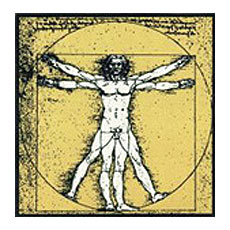
\includegraphics[width=1cm]{img/logoLEO.jpg}
  Scuola Leonardo Da Vinci (Firenze)
}

\author[Stefano Martina]{
  %\\[0.2cm]
  \textbf{Stefano MARTINA}\\
  {\small stefano.martina@gmail.com}
}

\titlegraphic{\tiny
  \href{http://creativecommons.org/licenses/by-sa/4.0/}{
\includegraphics[width=1cm]{img/logoCC.png}}
  This work is licensed under a
  \href{http://creativecommons.org/licenses/by-sa/4.0/}{Creative
    Commons Attribution-ShareAlike 4.0 International License}.}


\title[Lesson 6]{\textbf{Lesson 6 - Boolean logic and iterations}}
\date[15/10/15]{\flushright 15 October 2015}

\begin{document}

\begin{frame}[plain]
  \titlepage
\end{frame}

\begin{frame}
  \frametitle{Boolean logic}
  \begin{block}{Predicate}
    A function
    $$
    P:X\rightarrow \{true,false\}
    $$
    from a certain set $X$ (for istance $\mr\times\mr$) to a truth value. Can be: \cc{<}, \cc{>},
    \cc{<=} ($\leq$), \cc{>=} ($\geq$), \cc{==} ($=$), \cc{!=} ($\neq$)
    
  \end{block}
  \begin{block}{Logical connective}
    Technically predicates in the set:
    $\{true,false\}\times\{true,false\}$ ($\{true,false\}$ for the
    negation), can connect different expressions together. can be:
    \cc{\&\&} ($\wedge$), \cc{||} ($\vee$), \cc{!} ($\neg$).
    \begin{center}
      \begin{tabular}{|c|c||c|c|c|}
        \hline
        $a$ & $b$ & $\neg a$ & $a\wedge b$ & $a\vee b$ \\
        \hline
        0 & 0 & 1 & 0 & 0 \\
        0 & 1 & 1 & 0 & 1 \\
        1 & 0 & 0 & 0 & 1 \\
        1 & 1 & 0 & 1 & 1 \\
        \hline
      \end{tabular}
    \end{center}
  \end{block}
\end{frame}
\begin{frame}
  \begin{block}{Boolean expression}
    An expression that produce a boolean value when evaluated (true,
    false). Can be composed from
    \begin{itemize}
    \item variables
    \item predicates
    \item connectives
    \item parenthesis
    \end{itemize}
  \end{block}
  for instance:
  \begin{itemize}
  \item \cc{a<3}
  \item \cc{(a>5) \&\& (a<10)}
  \item \cc{(a<b) || !(a>=10 \&\& b<=5)}
  \end{itemize}
\end{frame}

\begin{frame}
  \frametitle{Iterations}
  \begin{center}
    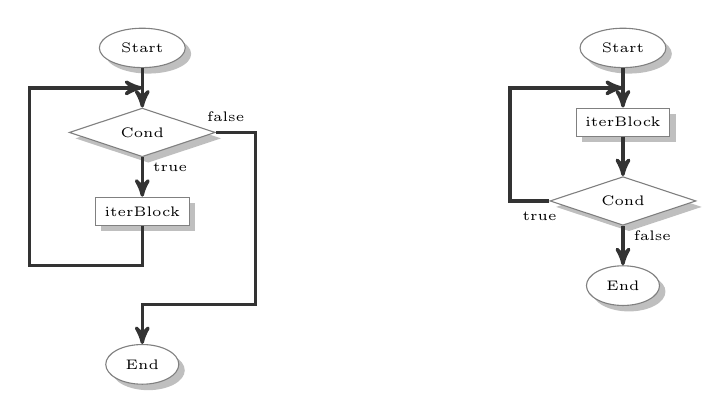
\begin{tikzpicture}[node distance=5mm, font=\tiny, auto]
      \node(start1) [fStartEnd] {Start};
      \node(selection1) [fSelection, below=of start1] {\cc{Cond}};
      \draw [arrow] (start1) -- (selection1);
      \node(iterBlock1) [fProcess, below=of selection1] {\cc{iterBlock}};
      \draw [arrow] (selection1) -- node [near start] {true} (iterBlock1);
      \node(end1) [fStartEnd, below=15mm of iterBlock1] {End};
      \draw [arrow] (iterBlock1)
      -- ($ (iterBlock1.south) - (0,5mm) $)
      -| ($ (selection1.west) - (5mm,0) $)
      |- ($ (selection1.north) + (0,2.5mm) $);
      \draw [arrow] (selection1)
      -- node [near start] {false} ($ (selection1.east) + (5mm,0) $)
      |- ($ (end1.north) + (0,5mm) $)
      -- (end1);
      
      \node(start2) [fStartEnd, right=50mm of start1] {Start};
      \node(iterBlock2) [fProcess, below=of start2] {\cc{iterBlock}};
      \draw [arrow] (start2) -- (iterBlock2);
      \node(selection2) [fSelection, below=of iterBlock2] {\cc{Cond}};
      \draw [arrow] (iterBlock2) -- (selection2);
      \draw [arrow] (selection2) 
      -- node [near start] {true} ($ (selection2.west) - (5mm,0) $)
      |- ($ (iterBlock2.north) + (0,2.5mm) $);
      \node(end2) [fStartEnd, below=of selection2] {End};
      \draw [arrow] (selection2) -- node [near start] {false} (end2);
    \end{tikzpicture}
  \end{center}
\end{frame}

\end{document}
